% !TeX root = ../main.tex

\section{Diskussion}

\begin{frame}{Diskussion}
    \begin{itemize}
        \item seit 2000 im Einsatz $\to$ heute etabliertes SSO-System~\cite{shibbolethShibbolethConsortium2024}
        
        \pause

        \item Open Source, grundsätzlich kostenfrei~\cite{shibbolethMembership}
        \item Angebot kostenpflichtiger Mitgliedschaften durch \emph{Shibboleth Consortium}~\cite{shibbolethMembership, shibbolethShibbolethConsortium2024}
        \begin{itemize}
            \item Support, weitere Partizipationsmöglichkeiten
            \item Beitrag basierend auf Art \& Größe der Institution~\cite{shibbolethMembership, shibbolethShibbolethConsortium2024}
            \item bspw. DFN, Stanford University, University of Oxford, MIT~\cite{shibbolethOurMembers2024}
        \end{itemize}

        \pause

        \item Unterstützung von Standardprotokollen\\
            bspw. SAML, OpenID Connect \& LDAP~\cite{cantorConsortiumFAQShibboleth2023, overtsoftwareAzureADADFS2022}
        \item Windows-unabhängig, dezentral~\cite{overtsoftwareAzureADADFS2022}
    \end{itemize}
\end{frame}


\begin{frame}{Diskussion II}
    \begin{itemize}
        \item nicht nur für interne Zugriffsverwaltung und Authentifizierung
        \item[$\Rightarrow$] Austausch von Authentifizierungsdaten von \alert{föderierten} Identitäten zwischen (externen) Organisationen~\cite{cantorConsortiumFAQShibboleth2023}
    \end{itemize}

    \begin{figure}
        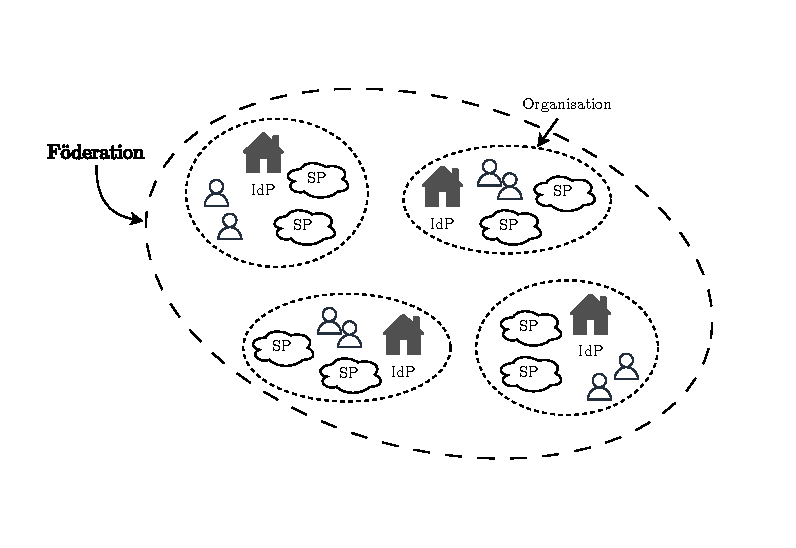
\includegraphics[height=4.3cm, clip, trim=0.7cm 1.3cm 1.0cm 1.3cm]{../assets/federation.drawio.pdf}
        \caption{Föderation~\cite[vgl.][]{switchFederation2025}}
    \end{figure}
    \vspace{-0.5cm}
\end{frame}



\begin{frame}{Alternativen}
    \begin{itemize}
        \item \emph{Active Directory} (AD)
        \begin{itemize}
            \item On-Premise, v.a. Windows-Umgebungen~\cite{sommergutWasSindUnterschiede2019}
            \item komplexe Einrichtung, kein Web-basiertes SSO
        \end{itemize}

        \pause

        \item \emph{Azure Active Directory} (AAD) / \emph{Microsoft Entra ID}
        \begin{itemize}
            \item Cloud-basiert, Microsoft-abhängig
            \item v.a. bei vollständiger Integration in Microsoft-Ökosystem~\cite{sommergutWasSindUnterschiede2019}
        \end{itemize}

        \pause

        \item weitere kostenpflichtige, Cloud-basierte Alternativen mit unterschiedlichem Fokus
        \begin{itemize}
            \item bspw. \emph{Okta}, \emph{OneLogin}, \emph{Ping Identity}~\cite{oktaSecureSingleSignOn, oneloginErweiterteAuthentifizierung, pingidentityFunktionenPingIdentityPlattform}
        \end{itemize}
    \end{itemize}
\end{frame}


\begin{frame}{Zukunft}
    \href{https://shibboleth.atlassian.net/wiki/spaces/DEV/pages/3503423489/Project+Roadmap}{\emph{Shibboleth Project Roadmap for 2024-2027}}

    \begin{itemize}
        \item passwortlose Authentifizierung\\bspw. mittels FIDO, WebAuthn \& Passkeys
        \item \emph{Digital Wallet}, \emph{Verified Credentials}
        \item Verbesserung der Dokumentation und Konfiguration für IdPs
        \item Neukonzeption der Service Provider (V4)\\$\to$ Plugin für IdPs
        \item Verbesserung des IdP-UI für Nutzende und Administrierende
        \item Unterstützung von \href{https://openid.net/foundation/}{\emph{OpenID Federation}}~\cite{shibbolethDevelopmentCenterProject2024}
    \end{itemize}
\end{frame}
